\documentclass[11pt,a4paper]{article}
\usepackage[T1]{fontenc}
\usepackage{lmodern}
\usepackage[spanish]{babel}
\usepackage[margin=2.35cm]{geometry}
\usepackage{graphicx}
\usepackage{array}

\newcolumntype{L}[1]{>{\raggedright\arraybackslash}p{#1}}
\setlength{\parindent}{0pt}
\setlength{\parskip}{5pt plus 1pt}
\setlength{\emergencystretch}{2em}

\begin{document}
{\small Universidad Técnica Estatal de Quevedo \par
Facultad de Ciencias de la Computación · Carrera de Software \par
Aplicaciones Distribuidas (ISR-701) · Aporte práctico de la Unidad I\par}
\vspace{0.65cm}
{\LARGE\bfseries AforoSeguro\par}
\vspace{0.15cm}
{\large Informe técnico de revisión posterior\par}
\vspace{0.2cm}
{\small Sesión del 23 de noviembre de 2026 · Usuario del repositorio: \texttt{CarlosManotoa007}\par}

\section*{Implementación registrada}
El prototipo usa Java RMI para que las puertas soliciten una admisión al coordinador. El servidor crea el registro en el puerto 1099, publica el objeto remoto con el nombre \texttt{Aforo} y recibe llamadas a \texttt{SumarAforo()}. RMI delimita y codifica cada invocación y su respuesta. El cliente usa el stub generado por RMI y captura las excepciones de comunicación.

El último commit centraliza el contador en el coordinador. El método \texttt{synchronized} protege en una sola sección crítica la comprobación del límite y el incremento. La respuesta devuelve el total actualizado si se permite la entrada, o \texttt{-1} si se alcanzó el límite. Los tres clientes hacen dos intentos cada uno. El límite es fijo y vale 5.

\section*{Evolución del repositorio}
\begingroup
\small
\renewcommand{\arraystretch}{1.23}
\begin{tabular}{@{}L{1.8cm}L{2.75cm}L{\dimexpr\linewidth-4.55cm-4\tabcolsep\relax}@{}}
\hline
\textbf{Commit} & \textbf{Hora (UTC$-$5)} & \textbf{Avance comprobable}\\
\hline
\texttt{fb6f14c} & 08:33:12 & Captura de desconexión y estructura inicial.\\
\texttt{51cc3dd} & 09:32:51 & Archivos iniciales del cliente, servidor e implementación remota.\\
\texttt{5e8e69d} & 09:56:05 & Intercambio RMI ejecutable. En dos lanzamientos posteriores, cada cliente volvió a contar de 1 a 5 porque enviaba su propio total.\\
\texttt{6c0dc2f} & 10:31:54 & Tres clientes y contador global sincronizado con rechazo al alcanzar el límite. Commit posterior al cierre de las 10:30 indicado por el estudiante.\\
\hline
\end{tabular}
\endgroup

\section*{Alcance de la entrega}
El historial disponible contiene cuatro commits. El mensaje inicial, «escenario E0», no incluye un código de sesión. Los mensajes posteriores tampoco muestran un código de sesión identificable. El repositorio original contiene una captura parcial de E0 y carece de la configuración externa, las bitácoras, el README, el informe y la carátula del SGA. La hora del commit es verificable en Git. La hora del \textit{push} y la entrega en el SGA quedan sin verificar.

Solicito que, si la guía permite revisar el avance previo al cierre, se valore el intercambio remoto de \texttt{5e8e69d}. Si se admite revisar el último commit, también se puede reproducir el uso del contador compartido y el rechazo por aforo completo.

\newpage
\section*{Escenarios y evidencia}
\begingroup
\small
\renewcommand{\arraystretch}{1.25}
\begin{tabular}{@{}>{\bfseries}L{1cm}L{2.65cm}L{\dimexpr\linewidth-3.65cm-4\tabcolsep\relax}@{}}
\hline
Caso & \textbf{Captura} & \textbf{Observación e interpretación}\\
\hline
E0 & Figura \ref{fig:e0} & Windows muestra «No conectado». La imagen carece de la lista de adaptadores, el usuario, el nombre de equipo y la fecha y hora visibles. Está en el primer commit.\\
E1 & Sin captura de sesión & Comprobación posterior parcial. Con un coordinador limpio, P1 obtuvo 1 y 2, P2 obtuvo 3 y 4 y P3 obtuvo 5 y un rechazo. La secuencia demuestra un contador compartido. Las operaciones de salida y estado quedaron pendientes.\\
E2 & Sin captura de sesión & Comprobación posterior parcial. La sexta entrada fue rechazada con «Aforo lleno» al alcanzar el límite implementado de 5. La prueba exigida usa un límite de 10 e incluye la autenticación, que quedó pendiente.\\
E3 & Sin captura de sesión & En una comprobación posterior, 30 hilos liberados juntos sobre un coordinador reiniciado obtuvieron 5 admisiones y 25 rechazos. Una llamada adicional devolvió \texttt{-1}. La prueba se hizo con un auxiliar externo al repositorio y con límite 5. El modo inseguro y \texttt{PruebaCarga} quedaron pendientes.\\
E4 & Sin captura de sesión & El código carece de latidos y de detección de puertas caídas o reactivadas.\\
E5 & Sin captura de sesión & Comprobación posterior parcial. Tras detener el coordinador, un nuevo lanzamiento de P1 informó «Error de comunicacion» por conexión rechazada a \texttt{localhost}. La puerta no confirmó ninguna entrada.\\
E6 & Sin captura de sesión & El código carece de relojes de Lamport, bitácoras y \texttt{OrdenTotal}. No se dispone de registros para identificar dos pares causales.\\
\hline
\end{tabular}
\endgroup

\begin{figure}[!h]
\centering
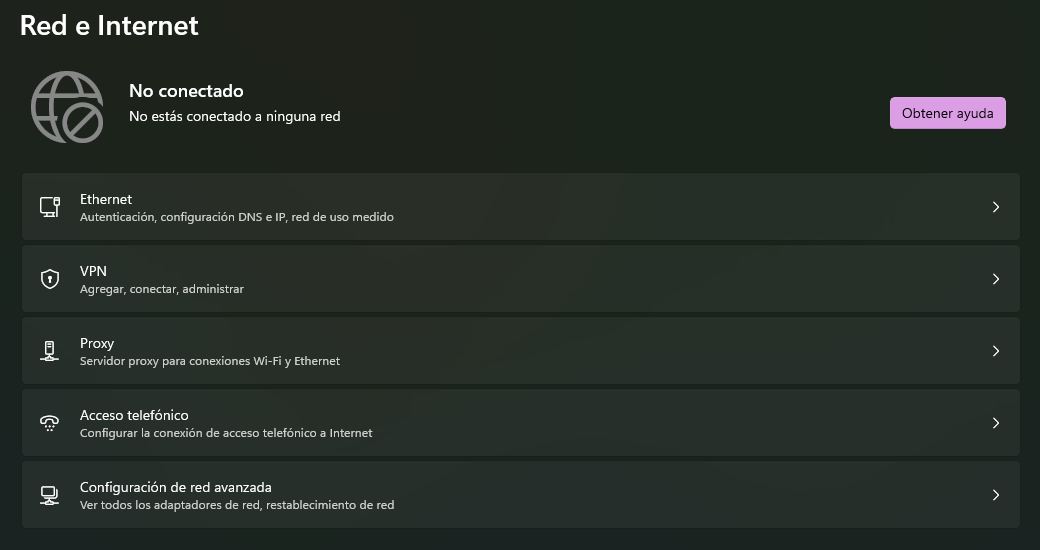
\includegraphics[width=0.87\linewidth]{../evidencia/Evidencia conexion desactivada.png}
\caption{Estado de red de Windows registrado en el primer commit.}
\label{fig:e0}
\end{figure}

\newpage
\section*{Preguntas de análisis}
\subsection*{1. Concurrencia y costo de la exclusión mutua}
En la comprobación posterior, las cinco admisiones produjeron los totales 1, 2, 3, 4 y 5. El método \texttt{synchronized} hace que cada hilo compruebe la capacidad y actualice el total antes de que otro entre en la sección crítica. El costo es que las llamadas concurrentes esperan su turno. El modo inseguro quedó pendiente, por lo que no se dispone de cifras comparativas. Si la comprobación y la escritura se separaran, dos solicitudes podrían observar la misma plaza libre y ambas recibir permiso.

\subsection*{2. Decisión al perder contacto con el coordinador}
Cuando P1 intentó conectarse con el coordinador detenido, mostró un error y terminó sin admitir a nadie. Desde la perspectiva de CAP, ante una separación de red esta política sacrificaría la disponibilidad de las admisiones para evitar autorizaciones basadas en un contador desactualizado. La prueba reprodujo la detención del servidor. Para el público, el efecto es que la fila se detiene. Para la administración, las puertas dejan de admitir personas sin autorización central.

\subsection*{3. Punto único de fallo}
El coordinador conserva todo el estado en memoria y lo pierde al reiniciar. Una mejora sería replicar el estado y elegir un coordinador activo mediante un quórum. La dificultad sería acordar el orden de las admisiones y confirmar cada actualización antes de responder. Si dos réplicas autorizan entradas con el mismo saldo de plazas o una solicitud se vuelve a aplicar en un reintento, el total puede quedar inconsistente.

\subsection*{4. Latencia y detección de fallos}
La temporización de la guía se relaciona con la falacia de que la latencia es cero. Con latidos cada 2 segundos y un umbral de 6, una demora que deje al coordinador más de 6 segundos sin recibir latidos puede producir una falsa caída. Con una demora constante de 7 segundos, el primer latido puede llegar después del umbral. Si luego los latidos llegan espaciados cada 2 segundos, por sí sola esa latencia constante no produciría nuevas caídas. El prototipo no implementa este mecanismo y el efecto descrito no se midió.
\end{document}
